\section{Class diagram}

\begin{flushleft}
Au niveau des méthodes contenues dans la partie serveur, il a d'abord fallu changer l'objet \textbf{WalletBasic} afin de stocker toutes les informations nécessaires pour l'extension, à savoir celles citées dans la partie base de données (premier paragraphe).
\end{flushleft}

\begin{flushleft}
Et ensuite, sachant que la plupart de l'implémentation se fera côté client, il a fallu rajouter deux méthodes. Une pour recevoir les données de la simulation que l'on va appeler \textbf{getConsumptionOfSimulation} et une autre pour vérifier que les données entrées sont normales, que l'on va appeler \textbf{isNormalData}.
\end{flushleft}

\begin{flushleft}
Finalement, j'ai dû rajouter l'id user en paramètre de \textbf{addConsumption} et \textbf{changeConsumption} afin de prévenir par mail si la donnée est anormale.
\end{flushleft}

\newpage
\begin{figure}[h]
\centering
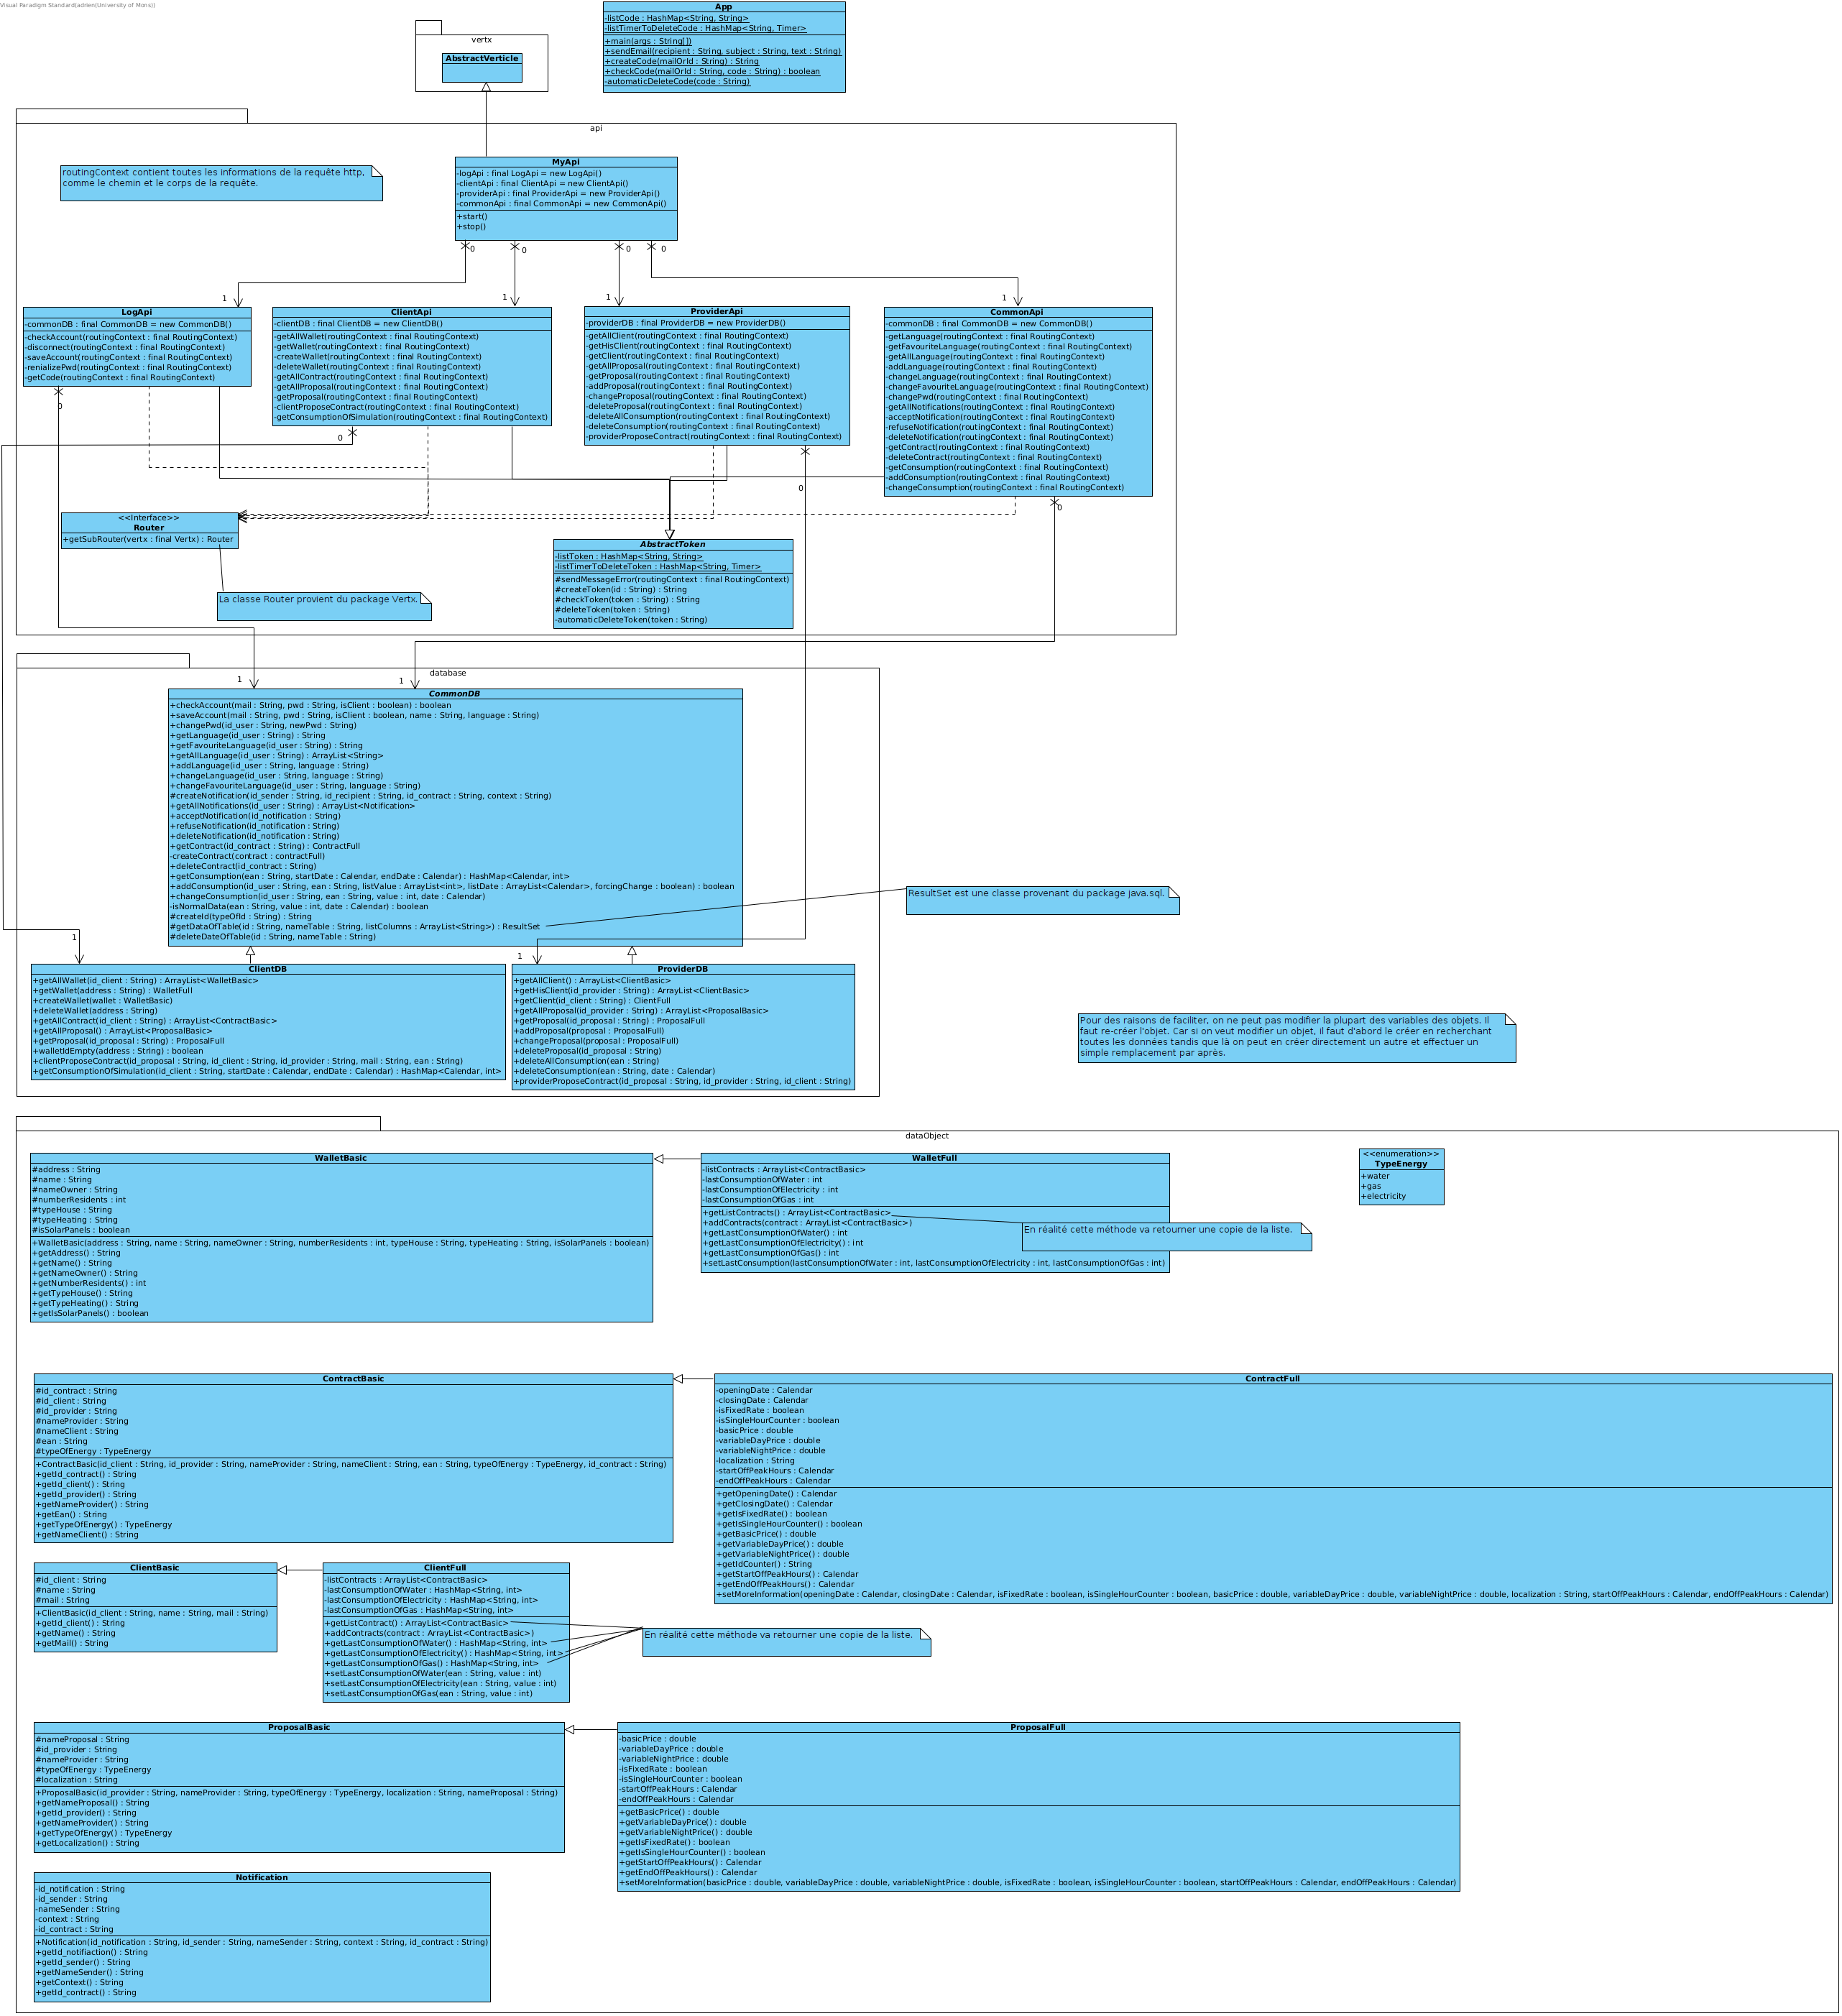
\includegraphics[width=1\textwidth]{extension-adrien/ClassDiagram/img/classDiagram.png}
\end{figure}
